% REV01 Wed 23 Jun 2021 06:24:38 WIB
% START Tue 04 May 2021 13:55:16 WIB

\chapter{IN WHICH THE ORPHAN MAKES HIS WILL}

The Secretary, working in the Dismal Swamp betimes next morning, was
informed that a youth waited in the hall who gave the name of Sloppy.
The footman who communicated this intelligence made a decent pause
before uttering the name, to express that it was forced on his
reluctance by the youth in question, and that if the youth had had
the good sense and good taste to inherit some other name it would have
spared the feelings of him the bearer.

‘Mrs Boffin will be very well pleased,’ said the Secretary in a
perfectly composed way. ‘Show him in.’

Mr Sloppy being introduced, remained close to the door: revealing
in various parts of his form many surprising, confounding, and
incomprehensible buttons.

‘I am glad to see you,’ said John Rokesmith, in a cheerful tone of
welcome. ‘I have been expecting you.’

Sloppy explained that he had meant to come before, but that the Orphan
(of whom he made mention as Our Johnny) had been ailing, and he had
waited to report him well.

‘Then he is well now?’ said the Secretary.

‘No he ain’t,’ said Sloppy.

Mr Sloppy having shaken his head to a considerable extent, proceeded
to remark that he thought Johnny ‘must have took ‘em from the Minders.’
Being asked what he meant, he answered, them that come out upon him and
partickler his chest. Being requested to explain himself, he stated that
there was some of ‘em wot you couldn’t kiver with a sixpence. Pressed to
fall back upon a nominative case, he opined that they wos about as
red as ever red could be. ‘But as long as they strikes out’ards, sir,’
continued Sloppy, ‘they ain’t so much. It’s their striking in’ards
that’s to be kep off.’

John Rokesmith hoped the child had had medical attendance? Oh yes, said
Sloppy, he had been took to the doctor’s shop once. And what did the
doctor call it? Rokesmith asked him. After some perplexed reflection,
Sloppy answered, brightening, ‘He called it something as wos wery
long for spots.’ Rokesmith suggested measles. ‘No,’ said Sloppy with
confidence, ‘ever so much longer than THEM, sir!’ (Mr Sloppy was
elevated by this fact, and seemed to consider that it reflected credit
on the poor little patient.)

‘Mrs Boffin will be sorry to hear this,’ said Rokesmith.

‘Mrs Higden said so, sir, when she kep it from her, hoping as Our Johnny
would work round.’

‘But I hope he will?’ said Rokesmith, with a quick turn upon the
messenger.

‘I hope so,’ answered Sloppy. ‘It all depends on their striking
in’ards.’ He then went on to say that whether Johnny had ‘took ‘em’
from the Minders, or whether the Minders had ‘took ’em from Johnny,
the Minders had been sent home and had ‘got ’em.’ Furthermore, that Mrs
Higden’s days and nights being devoted to Our Johnny, who was never out
of her lap, the whole of the mangling arrangements had devolved upon
himself, and he had had ‘rayther a tight time’. The ungainly piece of
honesty beamed and blushed as he said it, quite enraptured with the
remembrance of having been serviceable.

‘Last night,’ said Sloppy, ‘when I was a-turning at the wheel pretty
late, the mangle seemed to go like Our Johnny’s breathing. It begun
beautiful, then as it went out it shook a little and got unsteady, then
as it took the turn to come home it had a rattle-like and lumbered a
bit, then it come smooth, and so it went on till I scarce know’d which
was mangle and which was Our Johnny. Nor Our Johnny, he scarce know’d
either, for sometimes when the mangle lumbers he says, “Me choking,
Granny!” and Mrs Higden holds him up in her lap and says to me “Bide a
bit, Sloppy,” and we all stops together. And when Our Johnny gets his
breathing again, I turns again, and we all goes on together.’

Sloppy had gradually expanded with his description into a stare and a
vacant grin. He now contracted, being silent, into a half-repressed gush
of tears, and, under pretence of being heated, drew the under part of
his sleeve across his eyes with a singularly awkward, laborious, and
roundabout smear.

‘This is unfortunate,’ said Rokesmith. ‘I must go and break it to Mrs
Boffin. Stay you here, Sloppy.’

Sloppy stayed there, staring at the pattern of the paper on the wall,
until the Secretary and Mrs Boffin came back together. And with Mrs
Boffin was a young lady (Miss Bella Wilfer by name) who was better worth
staring at, it occurred to Sloppy, than the best of wall-papering.

‘Ah, my poor dear pretty little John Harmon!’ exclaimed Mrs Boffin.

‘Yes mum,’ said the sympathetic Sloppy.

‘You don’t think he is in a very, very bad way, do you?’ asked the
pleasant creature with her wholesome cordiality.

Put upon his good faith, and finding it in collision with his
inclinations, Sloppy threw back his head and uttered a mellifluous howl,
rounded off with a sniff.

‘So bad as that!’ cried Mrs Boffin. ‘And Betty Higden not to tell me of
it sooner!’

‘I think she might have been mistrustful, mum,’ answered Sloppy,
hesitating.

‘Of what, for Heaven’s sake?’

‘I think she might have been mistrustful, mum,’ returned Sloppy with
submission, ‘of standing in Our Johnny’s light. There’s so much trouble
in illness, and so much expense, and she’s seen such a lot of its being
objected to.’

‘But she never can have thought,’ said Mrs Boffin, ‘that I would grudge
the dear child anything?’

‘No mum, but she might have thought (as a habit-like) of its standing
in Johnny’s light, and might have tried to bring him through it
unbeknownst.’

Sloppy knew his ground well. To conceal herself in sickness, like a
lower animal; to creep out of sight and coil herself away and die; had
become this woman’s instinct. To catch up in her arms the sick child who
was dear to her, and hide it as if it were a criminal, and keep off all
ministration but such as her own ignorant tenderness and patience could
supply, had become this woman’s idea of maternal love, fidelity, and
duty. The shameful accounts we read, every week in the Christian year,
my lords and gentlemen and honourable boards, the infamous records of
small official inhumanity, do not pass by the people as they pass by
us. And hence these irrational, blind, and obstinate prejudices, so
astonishing to our magnificence, and having no more reason in them--God
save the Queen and Confound their politics--no, than smoke has in coming
from fire!

‘It’s not a right place for the poor child to stay in,’ said Mrs Boffin.
‘Tell us, dear Mr Rokesmith, what to do for the best.’

He had already thought what to do, and the consultation was very short.
He could pave the way, he said, in half an hour, and then they would go
down to Brentford. ‘Pray take me,’ said Bella. Therefore a carriage was
ordered, of capacity to take them all, and in the meantime Sloppy
was regaled, feasting alone in the Secretary’s room, with a complete
realization of that fairy vision--meat, beer, vegetables, and pudding.
In consequence of which his buttons became more importunate of public
notice than before, with the exception of two or three about the region
of the waistband, which modestly withdrew into a creasy retirement.

Punctual to the time, appeared the carriage and the Secretary. He sat
on the box, and Mr Sloppy graced the rumble. So, to the Three Magpies as
before: where Mrs Boffin and Miss Bella were handed out, and whence they
all went on foot to Mrs Betty Higden’s.

But, on the way down, they had stopped at a toy-shop, and had bought
that noble charger, a description of whose points and trappings had on
the last occasion conciliated the then worldly-minded orphan, and also a
Noah’s ark, and also a yellow bird with an artificial voice in him,
and also a military doll so well dressed that if he had only been of
life-size his brother-officers in the Guards might never have found him
out. Bearing these gifts, they raised the latch of Betty Higden’s door,
and saw her sitting in the dimmest and furthest corner with poor Johnny
in her lap.

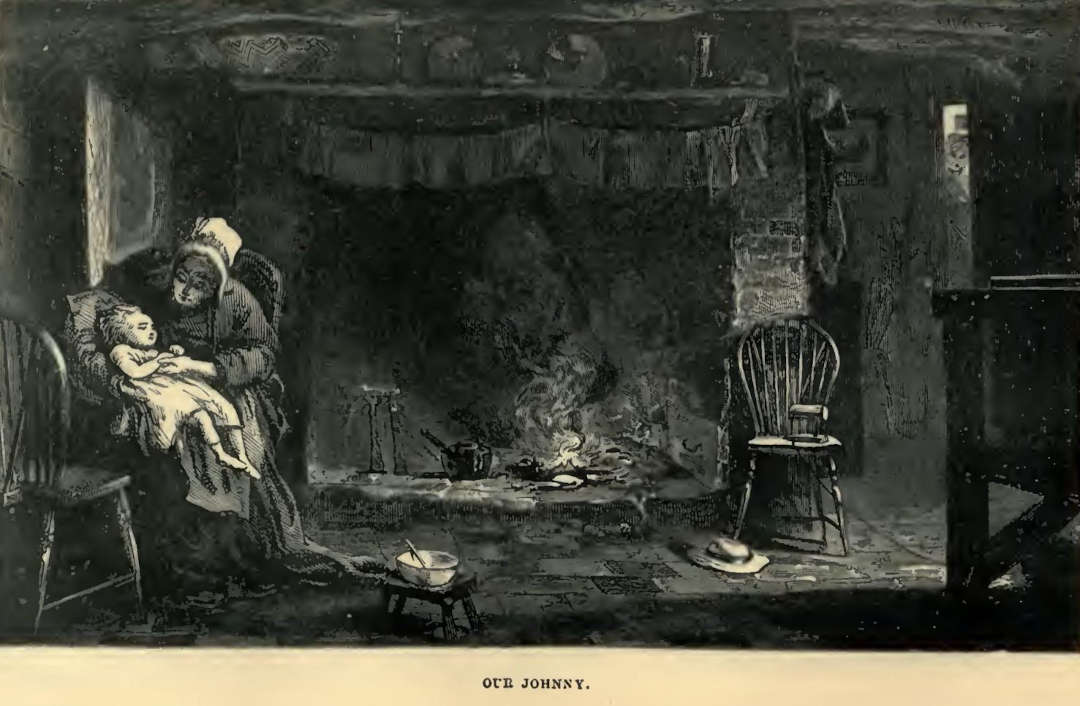
\includegraphics[scale=2.3]{02-09-01}

‘And how’s my boy, Betty?’ asked Mrs Boffin, sitting down beside her.

‘He’s bad! He’s bad!’ said Betty. ‘I begin to be afeerd he’ll not be
yours any more than mine. All others belonging to him have gone to
the Power and the Glory, and I have a mind that they’re drawing him to
them--leading him away.’

‘No, no, no,’ said Mrs Boffin.

‘I don’t know why else he clenches his little hand as if it had hold of
a finger that I can’t see. Look at it,’ said Betty, opening the wrappers
in which the flushed child lay, and showing his small right hand lying
closed upon his breast. ‘It’s always so. It don’t mind me.’

‘Is he asleep?’

‘No, I think not. You’re not asleep, my Johnny?’

‘No,’ said Johnny, with a quiet air of pity for himself; and without
opening his eyes.

‘Here’s the lady, Johnny. And the horse.’

Johnny could bear the lady, with complete indifference, but not the
horse. Opening his heavy eyes, he slowly broke into a smile on beholding
that splendid phenomenon, and wanted to take it in his arms. As it was
much too big, it was put upon a chair where he could hold it by the mane
and contemplate it. Which he soon forgot to do.

But, Johnny murmuring something with his eyes closed, and Mrs Boffin
not knowing what, old Betty bent her ear to listen and took pains to
understand. Being asked by her to repeat what he had said, he did so two
or three times, and then it came out that he must have seen more than
they supposed when he looked up to see the horse, for the murmur was,
‘Who is the boofer lady?’ Now, the boofer, or beautiful, lady was Bella;
and whereas this notice from the poor baby would have touched her of
itself; it was rendered more pathetic by the late melting of her heart
to her poor little father, and their joke about the lovely woman. So,
Bella’s behaviour was very tender and very natural when she kneeled on
the brick floor to clasp the child, and when the child, with a child’s
admiration of what is young and pretty, fondled the boofer lady.

‘Now, my good dear Betty,’ said Mrs Boffin, hoping that she saw her
opportunity, and laying her hand persuasively on her arm; ‘we have come
to remove Johnny from this cottage to where he can be taken better care
of.’

Instantly, and before another word could be spoken, the old woman
started up with blazing eyes, and rushed at the door with the sick
child.

‘Stand away from me every one of ye!’ she cried out wildly. ‘I see what
ye mean now. Let me go my way, all of ye. I’d sooner kill the Pretty,
and kill myself!’

‘Stay, stay!’ said Rokesmith, soothing her. ‘You don’t understand.’

‘I understand too well. I know too much about it, sir. I’ve run from
it too many a year. No! Never for me, nor for the child, while there’s
water enough in England to cover us!’

The terror, the shame, the passion of horror and repugnance, firing the
worn face and perfectly maddening it, would have been a quite terrible
sight, if embodied in one old fellow-creature alone. Yet it ‘crops
up’--as our slang goes--my lords and gentlemen and honourable boards, in
other fellow-creatures, rather frequently!

‘It’s been chasing me all my life, but it shall never take me nor mine
alive!’ cried old Betty. ‘I’ve done with ye. I’d have fastened door and
window and starved out, afore I’d ever have let ye in, if I had known
what ye came for!’

But, catching sight of Mrs Boffin’s wholesome face, she relented, and
crouching down by the door and bending over her burden to hush it, said
humbly: ‘Maybe my fears has put me wrong. If they have so, tell me, and
the good Lord forgive me! I’m quick to take this fright, I know, and my
head is summ’at light with wearying and watching.’

‘There, there, there!’ returned Mrs Boffin. ‘Come, come! Say no more of
it, Betty. It was a mistake, a mistake. Any one of us might have made it
in your place, and felt just as you do.’

‘The Lord bless ye!’ said the old woman, stretching out her hand.

‘Now, see, Betty,’ pursued the sweet compassionate soul, holding the
hand kindly, ‘what I really did mean, and what I should have begun by
saying out, if I had only been a little wiser and handier. We want to
move Johnny to a place where there are none but children; a place set
up on purpose for sick children; where the good doctors and nurses pass
their lives with children, talk to none but children, touch none but
children, comfort and cure none but children.’

‘Is there really such a place?’ asked the old woman, with a gaze of
wonder.

‘Yes, Betty, on my word, and you shall see it. If my home was a better
place for the dear boy, I’d take him to it; but indeed indeed it’s not.’

‘You shall take him,’ returned Betty, fervently kissing the comforting
hand, ‘where you will, my deary. I am not so hard, but that I believe
your face and voice, and I will, as long as I can see and hear.’

This victory gained, Rokesmith made haste to profit by it, for he saw
how woefully time had been lost. He despatched Sloppy to bring the
carriage to the door; caused the child to be carefully wrapped up; bade
old Betty get her bonnet on; collected the toys, enabling the little
fellow to comprehend that his treasures were to be transported with
him; and had all things prepared so easily that they were ready for
the carriage as soon as it appeared, and in a minute afterwards were
on their way. Sloppy they left behind, relieving his overcharged breast
with a paroxysm of mangling.

At the Children’s Hospital, the gallant steed, the Noah’s ark, yellow
bird, and the officer in the Guards, were made as welcome as their
child-owner. But the doctor said aside to Rokesmith, ‘This should have
been days ago. Too late!’

However, they were all carried up into a fresh airy room, and there
Johnny came to himself, out of a sleep or a swoon or whatever it was,
to find himself lying in a little quiet bed, with a little platform over
his breast, on which were already arranged, to give him heart and urge
him to cheer up, the Noah’s ark, the noble steed, and the yellow bird;
with the officer in the Guards doing duty over the whole, quite as much
to the satisfaction of his country as if he had been upon Parade. And at
the bed’s head was a coloured picture beautiful to see, representing as
it were another Johnny seated on the knee of some Angel surely who loved
little children. And, marvellous fact, to lie and stare at: Johnny had
become one of a little family, all in little quiet beds (except two
playing dominoes in little arm-chairs at a little table on the hearth):
and on all the little beds were little platforms whereon were to be
seen dolls’ houses, woolly dogs with mechanical barks in them not very
dissimilar from the artificial voice pervading the bowels of the yellow
bird, tin armies, Moorish tumblers, wooden tea things, and the riches of
the earth.

As Johnny murmured something in his placid admiration, the ministering
women at his bed’s head asked him what he said. It seemed that he wanted
to know whether all these were brothers and sisters of his? So they told
him yes. It seemed then, that he wanted to know whether God had brought
them all together there? So they told him yes again. They made out then,
that he wanted to know whether they would all get out of pain? So they
answered yes to that question likewise, and made him understand that the
reply included himself.

Johnny’s powers of sustaining conversation were as yet so very
imperfectly developed, even in a state of health, that in sickness they
were little more than monosyllabic. But, he had to be washed and tended,
and remedies were applied, and though those offices were far, far more
skilfully and lightly done than ever anything had been done for him in
his little life, so rough and short, they would have hurt and tired him
but for an amazing circumstance which laid hold of his attention. This
was no less than the appearance on his own little platform in pairs,
of All Creation, on its way into his own particular ark: the elephant
leading, and the fly, with a diffident sense of his size, politely
bringing up the rear. A very little brother lying in the next bed with a
broken leg, was so enchanted by this spectacle that his delight exalted
its enthralling interest; and so came rest and sleep.

‘I see you are not afraid to leave the dear child here, Betty,’
whispered Mrs Boffin.

‘No, ma’am. Most willingly, most thankfully, with all my heart and
soul.’

So, they kissed him, and left him there, and old Betty was to come back
early in the morning, and nobody but Rokesmith knew for certain how that
the doctor had said, ‘This should have been days ago. Too late!’

But, Rokesmith knowing it, and knowing that his bearing it in mind would
be acceptable thereafter to that good woman who had been the only light
in the childhood of desolate John Harmon dead and gone, resolved that
late at night he would go back to the bedside of John Harmon’s namesake,
and see how it fared with him.

The family whom God had brought together were not all asleep, but were
all quiet. From bed to bed, a light womanly tread and a pleasant fresh
face passed in the silence of the night. A little head would lift itself
up into the softened light here and there, to be kissed as the face went
by--for these little patients are very loving--and would then submit
itself to be composed to rest again. The mite with the broken leg was
restless, and moaned; but after a while turned his face towards Johnny’s
bed, to fortify himself with a view of the ark, and fell asleep. Over
most of the beds, the toys were yet grouped as the children had left
them when they last laid themselves down, and, in their innocent
grotesqueness and incongruity, they might have stood for the children’s
dreams.

The doctor came in too, to see how it fared with Johnny. And he and
Rokesmith stood together, looking down with compassion on him.

‘What is it, Johnny?’ Rokesmith was the questioner, and put an arm round
the poor baby as he made a struggle.

‘Him!’ said the little fellow. ‘Those!’

The doctor was quick to understand children, and, taking the horse,
the ark, the yellow bird, and the man in the Guards, from Johnny’s bed,
softly placed them on that of his next neighbour, the mite with the
broken leg.

With a weary and yet a pleased smile, and with an action as if he
stretched his little figure out to rest, the child heaved his body on
the sustaining arm, and seeking Rokesmith’s face with his lips, said:

‘A kiss for the boofer lady.’

Having now bequeathed all he had to dispose of, and arranged his affairs
in this world, Johnny, thus speaking, left it.



